\documentclass[]{article}
\usepackage{framed}
\usepackage{amsmath}
\usepackage{amssymb}
\usepackage{graphicx}
\usepackage{multicol}

\begin{document}


Chapter 1
D ` h d R l t`
Summary
Digraphs; Relations, using digraphs to illustrate relations, equivalence relations,
partial orders, relations and cartesian products.
%References: Epp Sections l0.l. 10.2, 10 3, 10.5 or B/1&:B Section 5.1.

\subsection*{Digraphs}
Some problems require that we dzrect the edges of a graph, from one endpoint to
the other, in order to express the relationship between the vertices A graph in
which every edge has a direction assigned to ir is called a \textit{\textbf{digraph}} (an abreviation
of directed graph). 

The directed edges are often called \textbf{arcs}.


\noindent\textbf{Example 1.1} Suppose we want to model a plan for traflic flow in part of a city,
where some streets allow trafiic flow in only one direction. 

For this model, a digraph would be appropriate, We would represent each road junction by a vertex; a one-way street from junction u to junction 1;, by an arc directed from u to UQ and a street allowing traffic flow in both directions between junctions rc and y, by two
arcs, one directed from x to y and the other from y to rv. 

An example is given in
Figure L17 where the direction of each arc is indicated by an arrow.
%-------- %
In a digraph we define directed paths and directed cycles as in graphs, but
with the added condition that arcs must be used in their correct direction, 

We say a digraph D is stongly corrected if for every pair of vertices x and y of D, there is a directed path from x to y and a directed path from y to x in D.
\begin{figure}[h!]
\centering
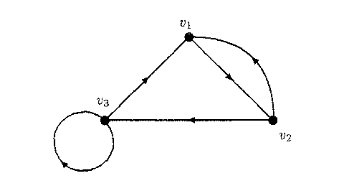
\includegraphics[width=0.7\linewidth]{./Digraph1}
\caption{}
\label{fig:Digraph1}
\end{figure}
%e 1.2: The relationship digraph of Example 1.3
Example 1.2 The digraph in Figure 1.1 contains a direcred path P = vamp; and
a directed cycle C : ugviug. lt is strongly connected.
Digraphs can be used to illustrate a variety of "one-way" relationships such as
predator-prey models in ecology, the scheduling of tasks in a manufacturing process.
family trees, flow diagrams for a computer program and many others.
\begin{figure}
\centering
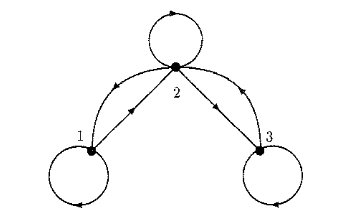
\includegraphics[width=0.7\linewidth]{./Digraph2}
\caption{}
\label{fig:Digraph2}
\end{figure}

